\documentclass[whitelogo]{TUD-report2020}

\usepackage{biblatex}
\addbibresource{report.bib}
\usepackage{booktabs}
\usepackage{colortbl}
\usepackage{xcolor}
\usepackage{changes}

\begin{document}
%% Use Roman numerals for the page numbers of the title pages and table of
%% contents.
\frontmatter

%% Uncomment following 19 lines for a cover with a picture on the lower half only
%\title[tudelft-white]{Title}
%\subtitle[tudelft-cyan]{Optional subtitle}
%\author[tudelft-white]{J.\ Random Author}
%\affiliation{Technische Universiteit Delft}
%\coverimage{cover.jpg}
%\titleoffsetx{10cm}
%\titleoffsety{10cm}
%\afiloffsetx{1cm}
%\afiloffsety{18cm}
%\covertext[tudelft-white]{
%    \textbf{Cover Text} \\
%    possibly \\
%    spanning 
%    multiple 
%    lines
%    \vfill
%    ISBN 000-00-0000-000-0
%}
%\makecover

%% Uncomment following 16 lines for a cover with a picture on the lower half only
\title[tudelft-white]{Title}
\subtitle[tudelft-black]{Optional subtitle}
\author[tudelft-white]{J.\ Random Author}
\affiliation{Technische Universiteit Delft}
\coverimage{tank.jpg}
\covertext[tudelft-white]{
    \textbf{Cover Text} \\
    possibly \\
    spanning 
    multiple 
    lines
    \vfill
    ISBN 000-00-0000-000-0
}
\setpagecolor{tudelft-cyan}
\makecover[split]


%% Include an optional title page.
\begin{titlepage}

\begin{center}

%% Insert the TU Delft logo at the bottom of the page.

%% Print the title in cyan.
{\makeatletter
\largetitlestyle\fontsize{64}{94}\selectfont\@title
%\largetitlestyle\color{tudelft-cyan}\Huge\@title
\makeatother}

%% Print the optional subtitle in black.
{\makeatletter
\ifx\@subtitle\undefined\else
    \bigskip
   {\tudsffamily\fontsize{22}{32}\selectfont\@subtitle}    
    %\titlefont\titleshape\LARGE\@subtitle
\fi
\makeatother}

\bigskip
\bigskip

door

\bigskip
\bigskip

{\makeatletter
\largetitlestyle\fontsize{26}{26}\selectfont 
\textbf{Groep 05}\\
\vspace{7mm}
M.D. Aarts (6044905) \\ 
C.S. Kalkman (5845394) \\ 
A. El Moubarik (5597617) \\ 
Z.R. Neuteboom (6010253) \\ 
S.J.J. Pufe (6071082)
\makeatother}


\bigskip
\bigskip


\vfill

\begin{tabular}{lll}
    Projectduur: & \multicolumn{2}{l}{9 februari 2026 -- 12 juni 2026} \\
    Projectbegeleider: & Prof.\ dr.\ ir.\ J.\ Pruijn, & TU Delft, supervisor \\
        & Dhr.\ H.\ Visser, & Kwartiermaker Project Maassluis\\
        & Dhr.\ W. van Baalen\ , & Waarnemend eigenaar Jansje
\end{tabular}

\bigskip
\bigskip
\emph{}

\bigskip
\bigskip
%\\[1cm]

%\centering{
\includegraphics{cover/logo_black}}


\end{center}
\begin{tikzpicture}[remember picture, overlay]
    \node at (current page.south)[anchor=south,inner sep=0pt]{
        
\includegraphics{cover/logo_black}
    };
\end{tikzpicture}

\end{titlepage}

\mainmatter
\let\cleardoublepage\clearpage



\chapter*{Samenvatting}
\setheader{Preface}

In samenwerking met loods M en haar stakeholders, zal een ontwerp gerealiseerd worden voor het historische transportschip Jansje. Hierbij is de harde eis dat de aandrijving in het nieuwe ontwerp draait op volledig hernieuwbare energie. Om tot dit ontwerp te komen, is eerst gekeken naar het vaarprofiel, en welke technische parameters hieruit voortvloeien. Door middel van een interview met de waarnemend eigenaar van Jansje is het operationeel profiel vastgesteld. 
\\\\
Daarna is er onderzoek gedaan naar de verschillende mogelijkheden voor energieopslagsystemen voor hernieuwbare energie. Dit is gedaan door middel van een uitgebreide literatuurstudie, een model, technische criteria en maatschappelijk relevante criteria. Er is gekeken naar zowel bestaande als nog experimentele techniek. De uitkomst hiervan is dat een combinatie van experimentele zeezoutbatterijen met lithium-ion batterijen de meest geschikte energiebron zal zijn. 
\\\\
Als laatst is onderzocht welke aandrijving het beste past bij het operationeel profiel van Jansje en de gekoze energiebron. Hieruit is voortgekomen dat een elektrische motor het meest geschikt is. Omdat er vele elektromotoren beschikbaar zijn, is ervoor gekozen om niet één elektromotor aan te bevelen, maar in plaats daarvan een set criteria mee te geven, waarmee er ten tijde van de daadwerkelijke implementatie de keuze gemaakt kan worden.





\tableofcontents

%% Use Arabic numerals for the page numbers of the chapters.
\mainmatter

\input{Hoofdstukken/Hoofdstuk i}
\input{Hoofdstukken/Hoofdstuk ii}
\input{Hoofdstukken/Hoofdstuk iii}
\input{Hoofdstukken/Hoofdstuk iv}
\input{Hoofdstukken/Hoofdstuk v}
\input{Hoofdstukken/Hoofdstuk vi}
\input{Hoofdstukken/Hoofdstuk 1}
\input{Hoofdstukken/Hoofdstuk 2}
\input{Hoofdstukken/Hoofdstuk 3}
\input{Hoofdstukken/Hoofdstuk 4}
\input{Hoofdstukken/Hoofdstuk 5}
\input{Hoofdstukken/Hoofdstuk 6}
\input{Hoofdstukken/Bijlage}
\chapter{Verdiepend experiment}
De zeezoutbatterij heeft nog geen nautische applicatie. Het is dus niet bekend hoe de batterij reageert op de schommelbewegingen die door de golven worden veroorzaakt. 
\section{Hoofdvraag}
Heeft de dynamica van golven invloed op het vermogen dat de batterij levert?
\section{Opstelling}
Voor dit experiment wordt een zeezoutbatterij (in het rood)  aan één kant van een hefboom (in het bruin) gezet. De andere kant van de hefboom zal handmatig heen en weer bewogen worden met variabele amplitude en frequentie. Op deze manier worden korte golven met hogere frequentie en lange golven met lagere frequentie nagebootst.
\begin{figure}[H]
    \centering
    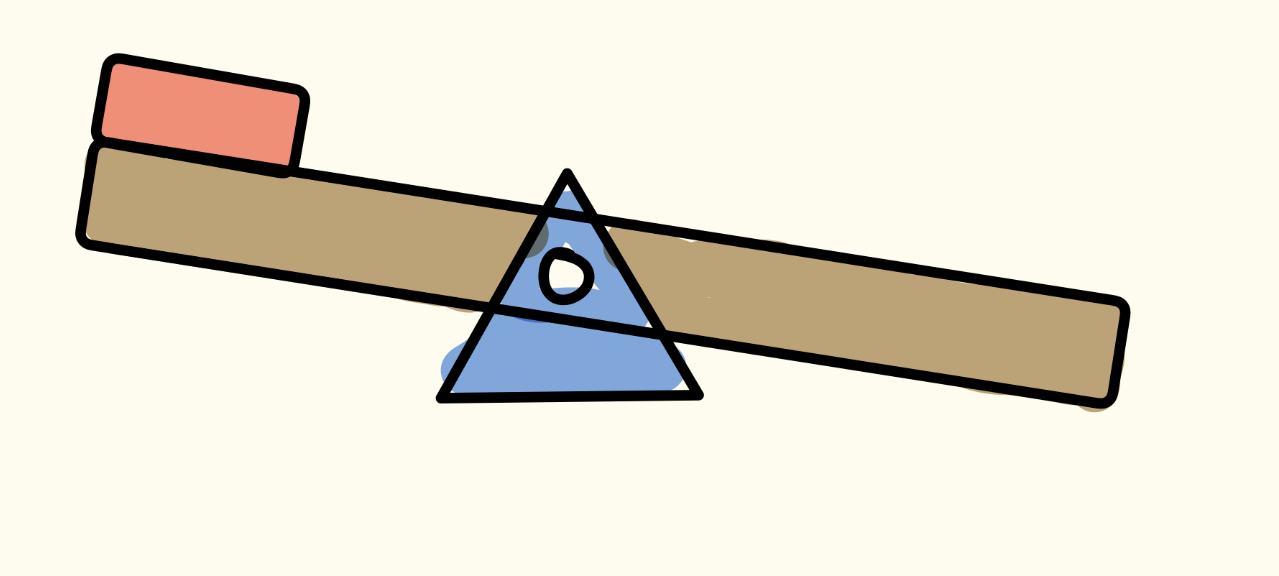
\includegraphics[width=0.5\linewidth]{opstelling.jpeg}
    \caption{Opstelling}
    \label{fig:Opstelling}
\end{figure}

\section{Voorbereiding}
Voor het experiment zijn de volgende onderdelen gebruikt:
\begin{itemize}
    \item \textbf{hefboom}, deze bestaat uit een houten plank met een as daardoorheen
    \item \textbf{multimeter voor stroom}, deze is in serie geschakeld met de batterij.
    \item{\textbf{multimeter voor spanning}, deze is in parallel geschakeld met de batterij en de \textit{load}.
    \item \textbf{\textit{load}}, deze zal bestaan uit een kleine elektromotor, om ervoor te zorgen dat het circuit de stroom ergens kwijt kan.
    \item \textbf{stopwatch} om een constante frequencie aan te houden tijdens de metingen.
\end{itemize}
In Figuur \ref{fig:Circuit} is een schema van de opstelling te zien en in Figuur \ref{fig:fysiek} de daadwerkelijke opstelling.
\begin{figure}[htbp]
    \centering
    \begin{minipage}{0.45\textwidth}
        \centering
        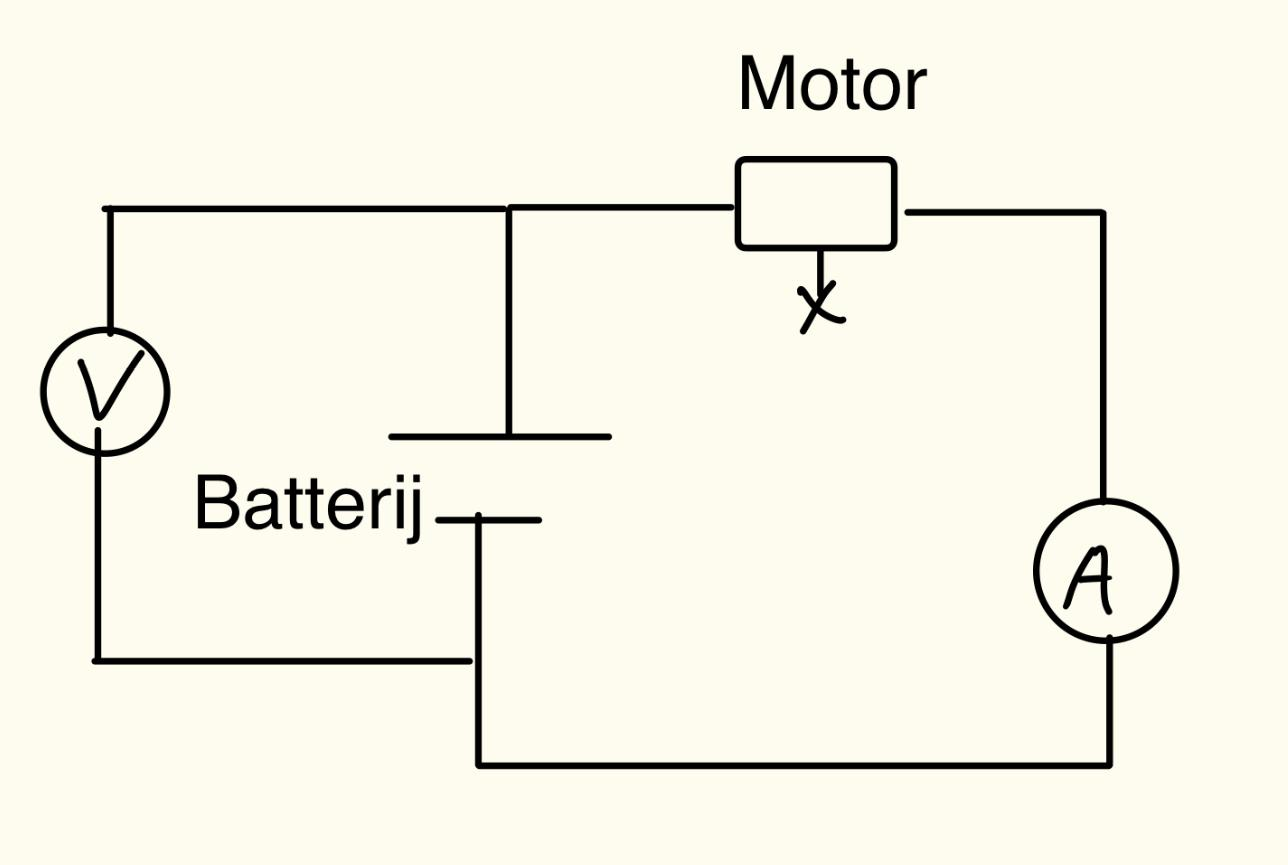
\includegraphics[width=\linewidth]{Circuit.jpeg}
        \caption{Circuit}
        \label{fig:Circuit}
    \end{minipage}\hfill
    \begin{minipage}{0.45\textwidth}
        \centering
        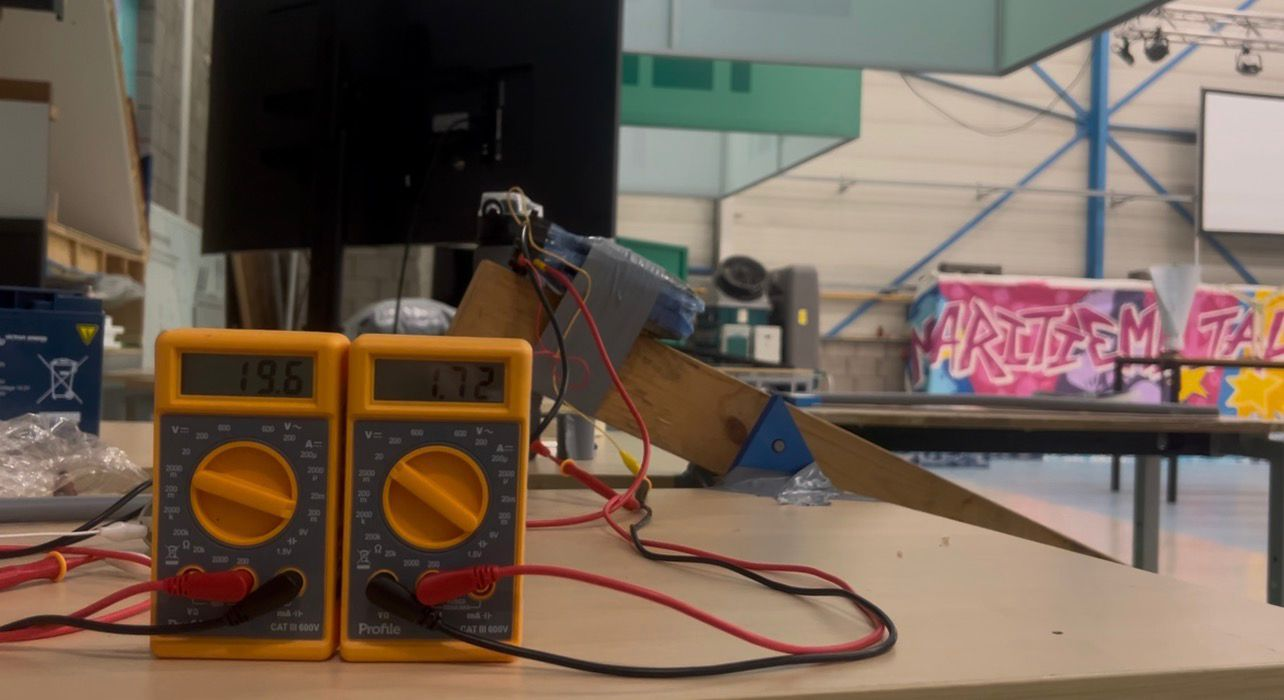
\includegraphics[width=\linewidth]{opstelling].jpeg}
        \caption{Opstelling fysiek}
        \label{fig:fysiek}
    \end{minipage}
\end{figure}

\section{Resultaten}
Met het experiment is de volgende data gerealiseerd:

\begin{table}[htbp]
\centering
\caption{Gemiddelde resultaten onderzoek }
\label{tab:experimental_results}
\begin{tabular}{l c S[table-format=2.3] S[table-format=1.3]}
\toprule
\textbf{Scenario} & \textbf{datapunten} & {\textbf{gemiddelde P (mW)}} & {\textbf{Std afwijking (mW)}} \\
\midrule
*Grote golven      & 60          & 33.664                 & 0.203                     \\
*Kleine golven     & 60          & 33.657                 & 0.172                     \\
\textbf{Statisch 0$^\circ$ (null)} & 60 & \textbf{33.398}     & \textbf{0.197}            \\
Statisch 45$^\circ$ & 59          & 33.442                 & 0.333                     \\
Statisch 90$^\circ$ & 60          & 33.164                 & 0.124                     \\
\bottomrule
\end{tabular}
\end{table}
*Bij de golf scenarios werd een frequentie van circa een trilling per seconde gebruikt, bij lichte golven een hoek van circa 20 graden en bij grote golven circa 45 graden.
\noindent
Deze tabel is een gemiddelde op basis van 60 datapunten met een tijdstap van een seconde, de volledige tabbellen zijn de te vinden in de bijlage [\ref{tab:static_0deg_data}].\\

\noindent
Het vermogen laat een lichte fluctuatie zien, deze fluctuatie is maximaal 0.8 procent van de nulmeting. Te observeren is dat de power afneemt van boven naar beneden in de tabel (bovenste meting is ook de eerste meting en de onderste de laatste meting), de hypothese hiervoor is dat de batterij iets leger is en daardoor (iets) minder krachtig is. 

\section{Conclusie}
Uit bovenstaande resultaten blijkt dat het verschil minder dan een procent is, in absolute termen 0.00026W. Hieruit wordt de conclusie getrokken dat golfbewegingen geen dan wel een verwaarloosbare invloed hebben op de praktische werking van de
batterij in de maritieme omgeving.

\section{Evaluatie}
Om de theorie te valideren dat de batterij leeg raakt en daardoor vermkogen verlies is, zou een volgend experiment gedaan moeten worden waar de batterij tussen sessies door naar het zelfde laadniveau gebracht moeten worden.
\chapter{Opladen van zeezoutbatterij HOEZO IS DIT HOOFDSTUK ENGELS?}

Tijdens het opladen is de volgende data gerealiseert:
\subsection{Setup}
For voltage measurement a multimeter is used.\\
For current measurement the gauge of the powersource is used.\\
Power source is an old (car)batterycharger. Can charge at 6V and 12V. We initialy set the power source to 6V.\\
surrounding temperature: 13degrees (outside temp, buienalarm, 17-5-26, 12:00, Baambrugge). battery is near an open window.\\
a test load (DC motor) is occacionaly used to determine if the load can be used for the actual test, and to read of the current with the multimeter, as it's probably more accurate than the gauge on the old charger.\\
During the experiment, at 11:54, two cables with small diameter are added to the circuits, to lower the charging current.

\subsection{SSB charging log}



start: 11:30
charge voltage:2.93v
charge current: 3.5A
\\\\
11:31: current keeps rising, now at 4 A\\
11:32: power shutoff, discharge current: 3.2A. discharge voltage 1.75\\
11:33: resume charging, 4A at 2.91V.\\
11:33: load checked, works.\\
11:35: heat check: no warmth discharge from the battery.\\
11:38: attempt to switch power source from 6V to 12V, current immediately rises to 6A (which is the max reading of the current gauge, so maybe more?). Actual voltage rises to 3.56.\\
11:38: switched back to 6V power source, so now charging at 2.87V, but current stays at 6+ A.\\
11:40: heat check of power soucre: slight warmth radiating from power source.\\
11:40: power source shut-off, attempt to let the load cycle. Battery doesn't yet have enough current. discharge power at steady 1.75V.\\
11:45: charging voltage has risen to 2.99V.\\
11:49: charging stopped. Power source is rated for 4A constant charging, where the battery continuously charged at 6+ A, for which the old power source wasn't designed.\\
11:49: heat check: no warmth discharge from battery. warmth discharge on power source slightly increased compared to previous measurement.\\
11:54: continue charging. Added some small cables inbetween to reduce charging current. Current is now at 2.4A, voltage at 4.04V.\\
11:55: power source makes small buzzing sound, probably also was there before, but didn't notice untill I checked.\\
11:55: tried to switch to 12V, current went to 4A, and voltage to 6.4V. However, as this is an old power source, charging at 4A continouusly will propbably damage it, so switched back to 6V.\\
11:57: charging at 4.17V, 2.2A.\\
11:58: voltage dropped to 3.85V, current still at 2.2A.\\
12:01: heat check: no warmth discharge from the battery, heat discharge from power source decreased. closed the window, it got cold and as the battery doesn't have any warmth discharge, no need for cooling.\\
12:01: voltage increased to 3.97V, current still 2.2A\\
12:03: voltage dropped to 3.89V, current 2.1A (current difference might be due to old equipment).\\
12:05: voltage increased to 3.91V, current 2.1A.\\
12:06: turned the multimeter upside down, then right side up, current now reads 4.01V.\\
12:12: steady charging at 4V, 2.1A. It also seems that the battery (4sacks in parallel, so 4 cells?) are rated for max 2.4A current, although the provided literature is a bit vague on what charging parameters to use. (is one sack one cell? And does "box of 4 blocks in parallel, 8 in series" mean box of 4 cells in parallel or 8 cells in series?\\
12:36: still charging at 4V, 2.1A.\\
12:36: heat check, seasalt battery has a very slight warmth, power source warmth decreased.\\
12:40: stopped charging, checked if battery can power load, which was succesfull.\\
12:42:'visual battery inspection. The leads of the cells seam to be rather soft, the clamps of the charger slightly deformed them.\\
12:45: amp test: output currently 0.27A.\\
12:52: resume normal charging. Due to slightly improves circuit, charging at 5.2V, 2.1A.\\
12:53: charged for approx 1hour, 0.27A.\\
13:03: charging at 5.3V,2.1A.\\
13:05 heat check: power source has negligible heat dissipation. Battery has slight heat dissipation, though only slightly sensible. Battery might have become a bit stiffer, although this has not been previously checked, and therefore can also not be the case. Small wires that where used start to heat up. might be wise to change them.\\
13:07: stop charging to swap out the small cables so they don't overheat.\\
13:08: discharge at 1.8V, which is quite good.\\
13:09: resumed charging, 5.4V at 2A. Swapped out the small cables for other ones of the same length, thickness, rating etc. old cables where cold already when I swapped them, and new ones where almost immediately the same temp as the old ones, so it seems to be just heat dissipation from the current, not accumulating heat, thus the cables do exactly what we want (act as additional resistance by dissipating heat). Connections of the multimeter have also improved, readings have become more stable.\\
13:41: steadily charging at 5.5V, 1.99A. slight local heat dissipation of the battery, though not even near concerning.\\
14:22: visual inspection: no notable differences.\\
14:22: heat inspection: heat dissipation from the battery increased more than previously measured. small cables are warm, but not concerning.\\
14:22: still charging at 5.5V, 2A. Even though the battery starts to warm up a bit, I would expect a drop in current when the battery is (almost) fully charged.\\
14:30: stopped charging.\\
14:30: voltage test: open circuit is 1.7V, closed circuit with load is 1.1V. Should the closed circuit lpad be 1.7V as well when fully charged?\\
14:33: resumed charging, 5.5V, 2A.\\
14:40: visual inspection: I noticed some hardened droplets on the top of the cells. They could just be adhesive used to seal the bags, but they might also be leakeage? Luckily, as this is a seasalt battery, there shouldn't be any harm to me.\\
14:45: stopped charging, ending the charging. The battery should be sufficiently charged for the upcomming test. \\
19:19: upon visual inspection: under certain light angle, slight yellow discoloration can be seen, although very slight. 


\subsection{Looking back}
The initial current of 6+ A at 3V is in line with the fact that the battery was deeply discharged. Also in line is the fact that, when the battery gains charge, the voltage increases and the current drops. According to the manufacturer, the charging time would be approximately eight hours. However, with three hours of charging, the battery should have enough charge for the experiment. Visualy inspecting the battery later, showed yellow coloring in the battery. According to the manufacturer this is due to crystals forming due to slight (local?) overcharging. however, In literature it is stated that a drop in charging current and rise in voltage should occur when the battery is near-full, which hasn't happened. This would lead to the conclusion that the battery might not have been optimaly functioning. However, this likely won't affect the experiment, as long as it keeps enough charge to complete the experiment.

\subsection{For the future}
The material of the poles are very soft, electrical clamps damage the surface and deform it. Furthermore, the poles aren't guarded, so putting them in a bag for traveling could create a current through the bag if the material is conducting. Therefore, for future experiments with similar cells I would advise to create a simple, hard plastic case and additional poles of a stronger metal.






%% Use letters for the chapter numbers of the appendices.
\appendix

%\input{appendix-a}

\printbibliography

\end{document}

